\documentclass[conference]{IEEEtran}
\IEEEoverridecommandlockouts
% The preceding line is only needed to identify funding in the first footnote. If that is unneeded, please comment it out.
\usepackage{cite}
\usepackage{amsmath,amssymb,amsfonts}
\usepackage{algorithmic}
\usepackage{graphicx}
\usepackage{textcomp}
\usepackage{xcolor}

\usepackage{mathtools}
\usepackage{amsmath}
\usepackage{amssymb}
\usepackage{caption}
\usepackage{subcaption}

\newcommand{\Part}[2]{\frac{\partial #1}{\partial #2}}
\newcommand{\Partt}[2]{\frac{\partial^2 #1}{\partial {#2}^2}}
\newcommand{\Partts}[3]{\frac{\partial^2 #1}{\partial {#2} \partial {#3}}}
\newcommand{\norm}[1]{\left\lVert#1\right\rVert}


\def\BibTeX{{\rm B\kern-.05em{\sc i\kern-.025em b}\kern-.08em
    T\kern-.1667em\lower.7ex\hbox{E}\kern-.125emX}}
\begin{document}

\title{Dense depth estimation from image pairs}

\author{\IEEEauthorblockN{Lucas Payne}
Supervisor: Richard Green\\
\IEEEauthorblockA{\textit{Department of Computer Science} \\
\textit{University of Canterbury}\\
\textit{Christchurch, New Zealand}\\
lcp35@uclive.ac.nz}}

\maketitle

\begin{abstract}
We compare variations of a variational method for dense
depth reconstruction from pairs of images.
The investigated class of methods are based on the minimization of a highly non-linear functional, which, given
a depth map estimate for camera one, measures the reprojection error between the corresponding
pixels in cameras one and two, assuming brightness constancy.
Important in this method is the use of a total-variation regularizer term, minimized with a method of Chambolle.
We assume that we have an accurate (and constant) intrinsic camera matrix,
our images are undistorted, and, importantly, that we have accurate camera pose estimations.
The main contribution of this paper is a small framework for the visualisation of iterative methods for this problem. We have
used this framework for the comparison of a simple brute-force method with a more sophisticated regularized scheme.

---todo: numerical result

\end{abstract}

\begin{IEEEkeywords}
depth estimation,
depth map,
ROF,
stereo,
total variation,
variational methods
\end{IEEEkeywords}

\section{Introduction}
In this paper, we compare variations of the method of Cremers \cite{dense_geometry} for dense
depth reconstruction from grayscale images. In particular we focus on the case of image pairs.
We assume (as in \cite{dense_geometry}) that we have an accurate (and constant) intrinsic camera matrix,
our images are undistorted, and, importantly, that we have accurate camera pose estimations.
The methodology is based on the minimization of a highly non-linear functional, which, given
a depth map estimate for camera one, measures the reprojection error between the corresponding
pixels in cameras one and two, assuming brightness constancy, as is assumed for the Horn-Schunck algorithm \cite{horn_schunck} for dense optical flow.
Important in this method is the use of a total-variation regularizer term, which penalizes noise in the depth map while retaining
depth discontinuities.
To minimize this functional, we use the method of Chambolle \cite{chambolle} --- designed for Rudin-Osher-Fatemi \cite{rof} denoising ---
combined with the splitting scheme of Zach et al. \cite{tv_optical_flow}, which in their paper is applied
to the problem of dense optical flow.

Following a short presentation of some important variational algorithms, we describe the method of Cremers
\cite{dense_geometry} and the total-variation optimization of Chambolle \cite{chambolle}.
Lastly, we present our main contribution: a small framework for the visualisation of iterative methods for the problem of
dense depth-map estimation from image pairs. We have used this framework for the comparison of a simple brute-force 
(and ineffective) method with a more sophisticated regularized scheme. ---todo: numerical results, discussion of future work

\section{Dense variational methods}
Here we give a short presentation of early variational methods used in computer vision ---
the Horn-Schunck and Rudin-Osher-Fatemi algorithms --- and a more recent related method of Zach et al. \cite{tv_optical_flow}
The methods outlined here serve as the algorithmic lineage of the method of Cremers et. al. \cite{dense_geometry}.
See the TUM lecture series by Cremers \cite{variational_lectures}, freely available online, for detailed descriptions of the mathematical underpinnings
and fundamental algorithms.

\subsection{The Horn-Schunck method for dense optical flow estimation with a regularized variational minimization.}
A well-known 1981 paper on optical flow estimation by Horn and Schunck \cite{horn_schunck} introduced what is now called the ``Horn-Schunck method'', one of the
first widespread variational algorithms used by the computer vision community
(See \cite{szeliski} for an introduction to the problem of optical flow estimation.) The Horn-Schunck method, when introduced, was unique in that
it computes a \textit{dense} field of motion vectors. The method is usefully formulated as a continuous optimization problem.
Given a stream of grayscale images $I^t : [0,1]^2 \rightarrow \mathbb{R}$, we would like to compute, for each point in the image at time $t$, a (space and time) velocity vector $(u,v,1)$
which which minimizes the directional derivative
    $$\nabla I^t \cdot(u, v, 1) = \Part{I^t}{x} u + \Part{I^t}{y}v + \Part{I^t}{t}.$$
This effectively finds the most likely ``motion vector'' which connects this point, as time goes on, to a point
in a subsequent image with the closest intensity value.
We can then formulate the functional
\begin{equation}
    E(u, v) = \int_0^1\int_0^1\left(\Part{I^t}{x} u(x,y) + \Part{I^t}{y}v(x,y) + \Part{I^t}{t}(x,y)\right)^2 \,dx\,dy,
\end{equation}
and our algorithm is simply the optimization problem
\begin{equation}\label{horn_schunck_unregularized}
    \min_{u,v}E(u, v).
\end{equation}
At this point, as in all variational optimization methods,
the essential conceptual work is done, and the rest of the work is in the choice of optimization strategy,
and our method of discretization. However, there is a fatal flaw in \eqref{horn_schunck_unregularized}.
Suppose that the brightness constancy assumption is fully satisfied; that is, we have $\nabla I^t \cdot (u, v, 1) = 0$
for ground truth motion vector $(u,v,1)$. We immediately see that this is one linear equation in two variables,
    $$u\Part{I^t}{x} + v\Part{I^t}{y} = -\Part{I^t}{t},$$
and that for any $u^*,v^*$ such that
    $$u^*\Part{I^t}{x} + v^*\Part{I^t}{y} = 0,$$
we have another solution, $(u + u^*, v + v^*)$ (see figure \ref{aperture_problem}). This is called the \textit{aperture problem} \cite{aperture_problem}, and is due to
the fact that the velocity vector field is estimated locally. The key modification of Horn and Schunck is the addition of a regularizer term which penalizes
high variation of the motion field, based on the observation that, except on object boundaries and occlusions, motion vector fields should be smooth. Their modified algorithm
solves the optimization problem
\begin{equation}\label{horn_schunck_regularized}
    \min_{u,v}\left\{E(u, v) + R(u,v)\right\},
\end{equation}
where $R(u,v)$ is the regularizer term
    $$\alpha^2\int_0^1\int_0^1\norm{u}^2 + \norm{v}^2\,dx\,dy,$$
for regularizer parameter $\alpha$ (the higher $\alpha$, the smoother the resulting vector field).
Quadratic data and regularizer terms are chosen in order to reduce the discretized Euler-Lagrange equations to a system of linear equations solved for
the global minimizer (see \cite{variational_calculus} and \cite{variational_lectures} for more information on variational calculus).
A quadratic regularizer, however, disproportionately penalizes discontinuities, such as across real object boundaries. We will
address this problem below.

\subsection{The Rudin-Osher-Fatemi (ROF) model for image denoising with total variation}
The problem of image denoising can be put in a global optimization
framework. We care here about the form of the optimization problem, rather than the application, and the ROF model turns out to be exactly
the same optimization required in the ``regularization step'' in \cite{tv_optical_flow}, \cite{dense_geometry}.
A cost function is formulated that penalizes ``noise'' and rewards closeness to the original (noisy) image. The algorithm then
consists of minimizing this cost function over all possible candidate ``denoised'' images. In fact, this algorithm is effectively the same
as the above Horn-Schunck method, utilizing a slightly different data term, with a more robust regularizer.

Let $I:[0,1]^2 \rightarrow \mathbb{R}$ be a square grayscale image with continuous domain, and
$I_{i,j}$ denote the intensity at pixel $(i, j)$ in the sampled discrete image.
One formulation of the continuous ROF cost function is
\begin{equation}\label{rof_continuous}
\begin{split}
    E(\hat{I}) &= \int_0^1\int_0^1 \frac{1}{2} \left(I(x,y) - \hat{I}(x,y)\right)^2 + \lambda \|\nabla \hat{I}(x,y)\| \,dx \,dy.
\end{split}
\end{equation}
The left-hand term in the integrand is the quadratic data term, penalizing differences from the original noisy image.
$\|\nabla \hat{I}(x,y)\|$ is a measure of the local variation of intensity at a point in the image.

A common finite difference approximation for $\nabla\hat{I}(x,y)$, valid for non-boundary pixels, is
\begin{equation}
    \hat{\nabla}I_{i,j} = \left(\frac{I_{i+1,j} - I_{i-1,j}}{2\Delta x}, \frac{I_{i,j+1} - I_{i,j-1}}{2\Delta y}\right)^T,
\end{equation}
where $\Delta x, \Delta y$ are pixel extents in the image domain. Where the original image is discontinuous, such as at edges,
this finite difference vector can be very large. Furthermore, the set of pixels whose finite-difference stencils extend over discontinuities is
\textit{not} neglible in the finite approximation of integral \eqref{rof_continuous}. A quadratic regularizer, such as
$\frac{\lambda}{2} \|\nabla \hat{I}\|^2$ will harshly penalize the appearance of sharp discontinuities, since a large value returned
by a finite difference is squared. The main idea behind the ROF model is to use the non-squared ``total-variation'' $\lambda \|\nabla \hat{I}\|$.
While this is notably more difficult to optimize (precluding the use of simple linear least squares), the final effect is a preservation
of isolated discontinuities such as edges and stripe patterns, while still penalizing large patches of interior noise. Notably, the ROF model can be solved by a non-linear diffusion process, performing gradient descent to solve the Euler-Lagrange
equations of the cost functional \cite{variational_calculus}. See their classic paper \cite{rof} for details, and \cite{variational_lectures} for a more recent discussion.

Fundamentally, dense variational methods such as \cite{horn_schunck} and \cite{dense_geometry} follow these same lines. First,
a cost functional of a image with continuous domain is formulated, penalizing unwanted properties of the solution. This cost functional is discretized,
and the algorithm outputs a discrete function (such as a denoised image, or a depth map, or an optical flow field) which minimizes the discrete cost function.
The majority of the complexity is in the method used to minimize (or attempt to minimize) this cost function, which could be highly non-linear.


% Two-dimensional areas of an image with high local variation
% are considered ``noisy''. Edges cause extremely high local variation --- in fact, an image with continuous domain may not be differentiable. However,
% finite difference approximations (such as the common ``forward difference''
% The important contribution of the ROF model
% is that this regularizer, which penalizes noise, is \textit{not} quadratic. A 

\subsection{Total-variation for dense optical flow estimation}
In \cite{tv_optical_flow}, Zach et al. formulate the optical flow problem
as a global optimization with non-quadratic data and regularizer terms.
This gives a modification
of the Horn-Schunck algorithm which is more robust to outliers and which tends to preserve motion discontinuities across object boundaries.
Zach et al.'s main contribution is their method of optimization,
which we will reproduce in the context of dense depth map estimation.
See their paper \cite{tv_optical_flow} for full details in the context of dense optical flow estimation.

\section{Total variation for depth map estimation from image pairs}
The paper by Cremer's et al. \cite{dense_geometry} applies the method of Zach et al. \cite{tv_optical_flow} to
the problem of dense depth-map
reconstruction from collections of (grayscale) images. For simplicity, we restrict our attention to the case of two images only ---
see \cite{dense_geometry} for details on the generalization. We assume (as in \cite{dense_geometry}) that we have an accurate (and constant) intrinsic camera matrix,
our images are undistorted, and, importantly, that we have accurate camera pose estimations. We describe here a slightly modified version of Cremer's method.

Let $C_1$ and $C_2$ denote the two cameras, $I_1$ and $I_2$ denote the two images, and let $h$ be the estimated depth map for $C_1$.
Our fully non-linear cost function is
\begin{equation}
\begin{split}
% E(h) &= \lambda \int_0^1\int_0^1{\Omega_0}\left\|I_1(\pi(\exp(\hat{\eta}_1)X(x,h)) - I_0(\pi(x))\right\|
%      + \|\nabla h\| \,dx\,dy,
E(h) &= \lambda \frac{1}{|\Omega^*|}\int_{\Omega^*}\left\|I_2(\text{reproj}(x,y)) - I_1(x,y)\right\|\,dx\,dy \\
     &+ \int_0^1\int_0^1\|\nabla h\| \,dx\,dy.
\end{split}
\end{equation}
which has TV-$L^1$ \cite{tv_optical_flow} data and regularizer terms. $\text{reproj}(x,y)$ is where the non-linear complexity is.
$x$ and $y$ denote image coordinates in $I_1$, and $h$ gives a transformation from these image coordinates to world-space,
given the camera pose of $C_1$. We can then project this point to the image space of $I_2$. $\Omega^* \subset [0,1]^2$
is defined as
\begin{equation}
    \Omega_0 \coloneqq \left\{(x,y) \in [0,1]^2 \mid \text{reproj}(x,y) \in [0,1]^2\right\}.
\end{equation}
Therefore, our data term is weighted over those pixels which have valid reprojections. Without the $1/|\Omega^*|$ factor
in the data term, our optimization would likely cause $h$ to be a constant function (giving zero regularizer cost), large enough such that
all reprojections are invalid (giving zero data cost) --- Weighting by $1/|\Omega^*|$ has been effective in our implementation.



Let $\rho(h) = \left\|I_1(\pi(\exp(\hat{\eta}_1)X(x,h)) - I_0(\pi(x))\right\|$. Since the data term is non-quadratic, we
cannot apply the ROF optimization method directly. However, we can introduce
an auxiliary depth map $h^\prime$ to separate the data and regularizer terms,
and introduce a penalizer for disparity between $h^\prime$ and $h$. The
new separable cost function is
\begin{equation}\label{separable_cost}
    \hat{E}_\theta(h, \hat{h}) = \int_\Omega \lambda \|\rho(h)\| + \frac{1}{2\theta}(h - \hat{h})^2 + \|\nabla \hat{h}\|.
\end{equation}
The parameter $\theta$ is set to some small constant.
The cost function $E_\theta$ is separated into functions of $h$ and $h^\prime$,
and $h$ and $h^\prime$ are alternately optimized in the following way:
\begin{itemize}
    \item For $h$ fixed, solve
        \begin{equation}\label{minh}
            \min_{h^\prime} \int_\Omega \lambda \|\nabla h^\prime\| + \frac{1}{2\theta}(h - h^\prime)^2\,dx
        \end{equation}
    using the ROF optimization methods.
    \item For $h^\prime$ fixed, solve
        \begin{equation}\label{minhhat}
            \min_h \int_\Omega \|\rho(h)\| + \frac{1}{2\theta}(h - h^\prime)^2\,dx.
        \end{equation}
        Since $\rho(h)$ measures point-wise reprojection error, this
        optimization can be done point-wise.
\end{itemize}
The ROF cost function \eqref{minh} can be minimized using the iterative method of Chambolle \cite{chambolle}. For completeness, we reproduce this
method here in the context of dense depth map estimation. We provide no proofs --- see \cite{chambolle} for full details.


% The quadratic term $\frac{1}{2\theta}(h-h^\prime)^2$, for small $\theta$, makes
% sure that the iteration makes ``small steps''.


\section{Visualization and dataset}
A visual tool for rapidly prototyping new dense reconstruction methods is provided.
We evaluate our method on the ``freiburg3\_long\_office\_household'' RGBD dataset, which contains accurate ground-truth camera poses, and
depth maps constructed using a Kinect sensor \cite{dataset} \cite{largescale}. Our tool allows these depth maps to be used as a drop-in replacement for the estimated
depth maps, to get a rough comparison against the ``ground truth''. Figure \ref{noisevis_computed} shows an example visual inspection of the output
of our total-variation algorithm.

\begin{figure}[htbp]
\begin{subfigure}[b]{0.5\textwidth}
\centerline{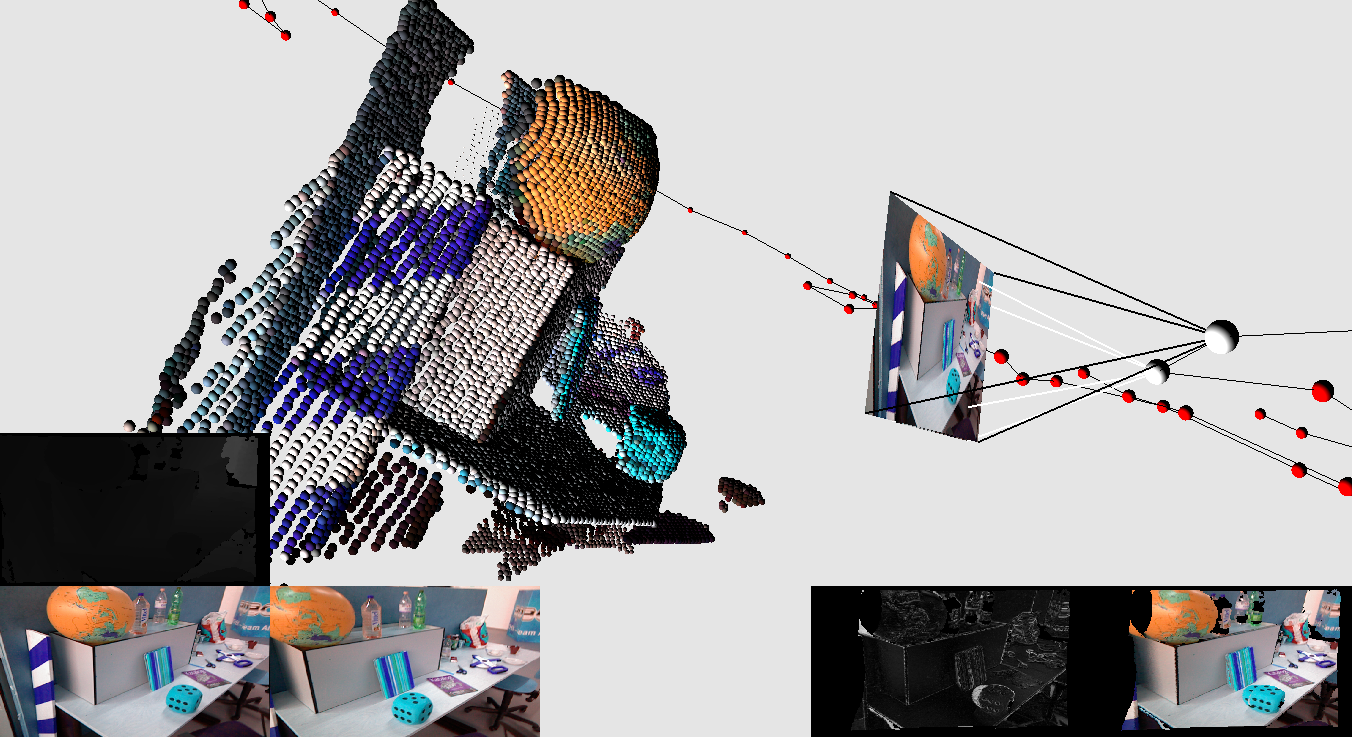
\includegraphics[width=\textwidth]{figures/cloud_groundtruth.png}}
\caption{Ground truth point cloud from the Kinect sensor}
\label{cloud_groundtruth}
\end{subfigure}
\begin{subfigure}[b]{0.5\textwidth}
\centerline{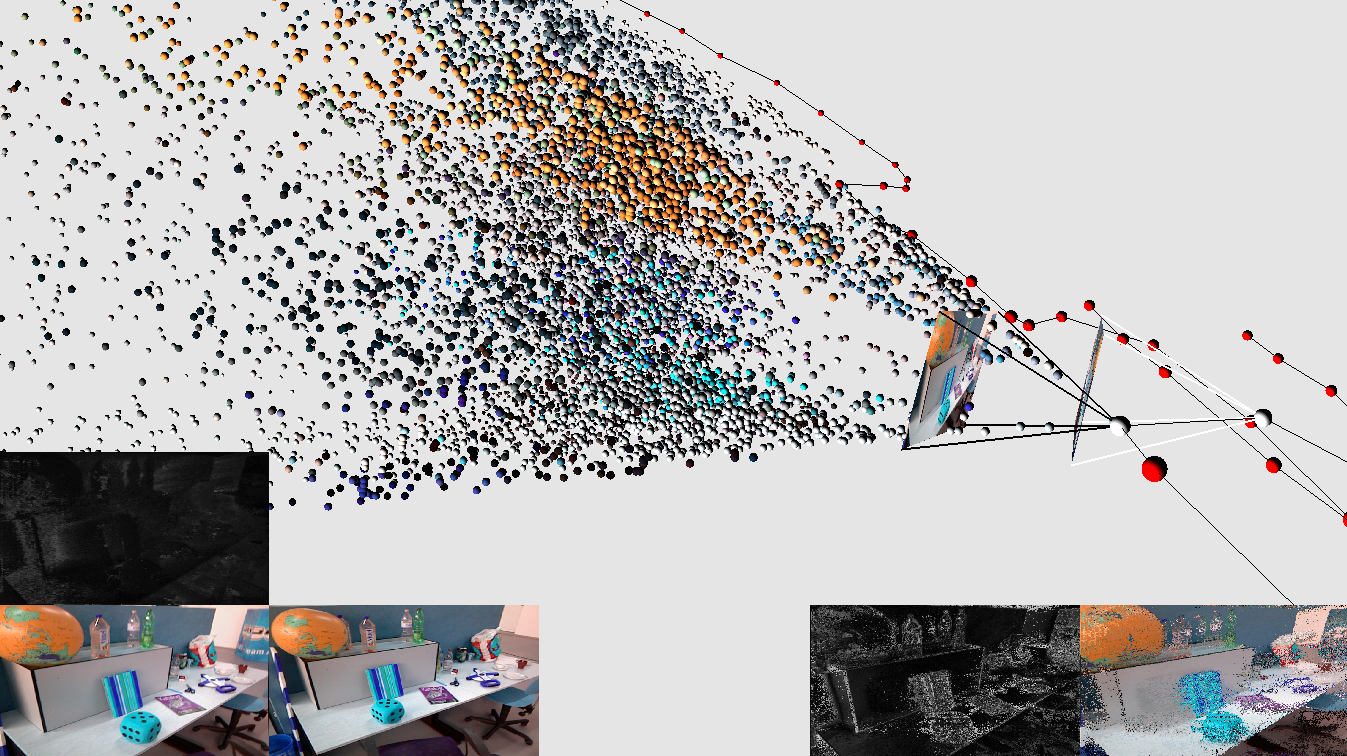
\includegraphics[width=\textwidth]{figures/cloud_noregularizer.png}}
\caption{Reconstruction estimate, computed without a regularizer. The reprojection-error-minimizing depth is chosen for each pixel with no regard to adjacent depths.}
\label{cloud_noregularizer}
\end{subfigure}
\begin{subfigure}[b]{0.5\textwidth}
\centerline{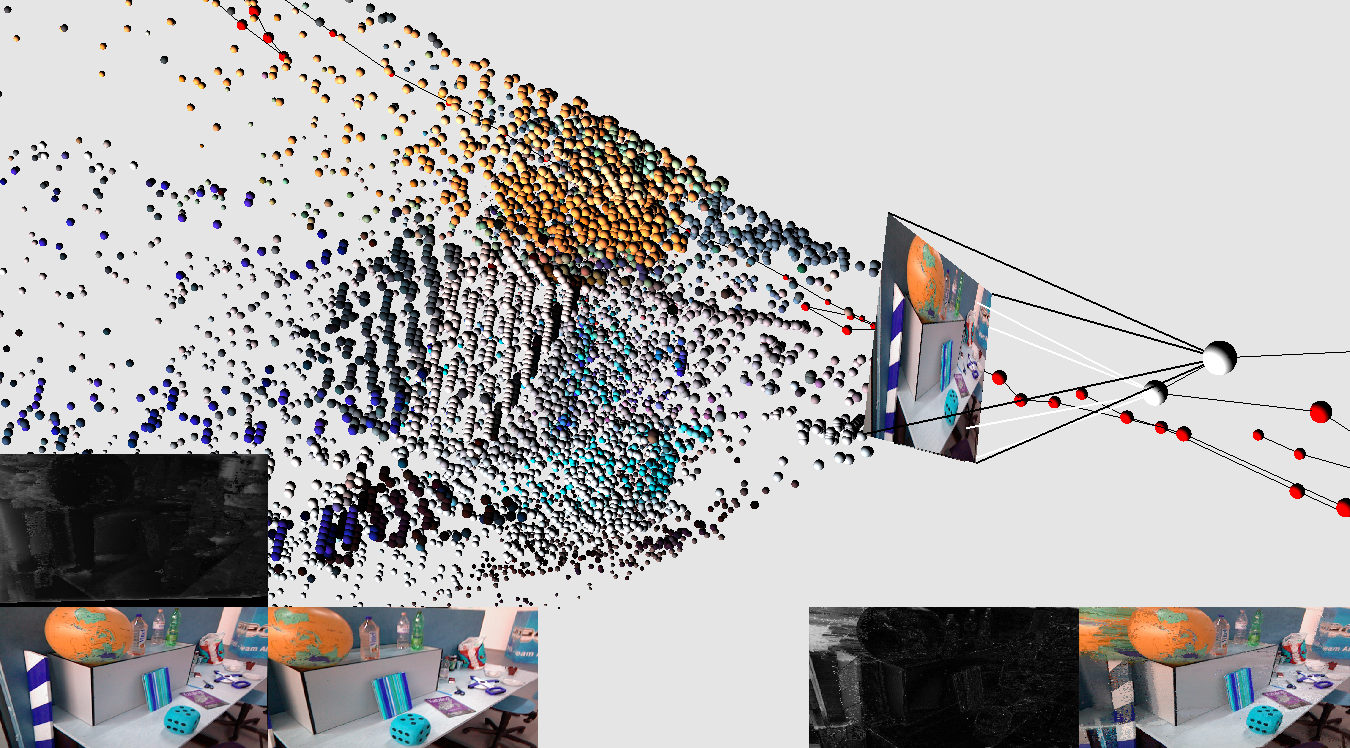
\includegraphics[width=\textwidth]{figures/cloud_computed.png}}
\caption{Reconstruction estimate, computed with a regularizer. Note that point clusters are preserved yet begin to form (noisy) surfaces.}
\label{cloud_computed}
\end{subfigure}
\end{figure}


Figure \ref{cloud_computed} displays some preliminary results, using heuristically determined parameters of $\theta$, $\lambda$, and $\tau$, and around 25 iterations.
Clearly this depth map is not satisfactory. However, it has some important qualitative features. Firstly, self-occlusion is captured for the
orange globe in the reprojection image, which is not captured by the brute-force method. Secondly, the point cloud clusters generally
toward the real object locations --- note the orange cluster near the globe. These results are compared to the ground truth point cloud shown
in figure \ref{cloud_groundtruth}.


\begin{figure}[htbp]
\begin{subfigure}[b]{0.5\textwidth}
\centerline{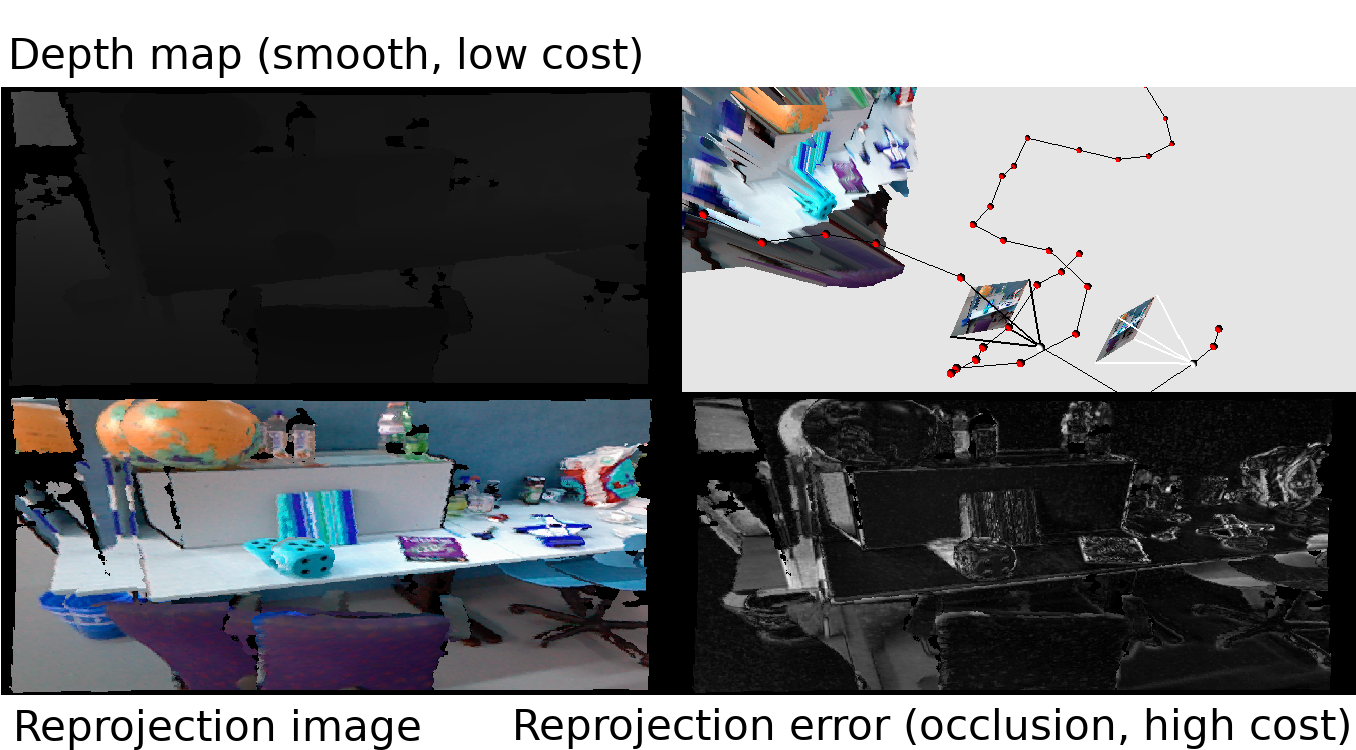
\includegraphics[width=\textwidth]{figures/noisevis_groundtruth_text.png}}
\caption{Ground truth depth data}
\label{noisevis_groundtruth}
\end{subfigure}
\begin{subfigure}[b]{0.5\textwidth}
\centerline{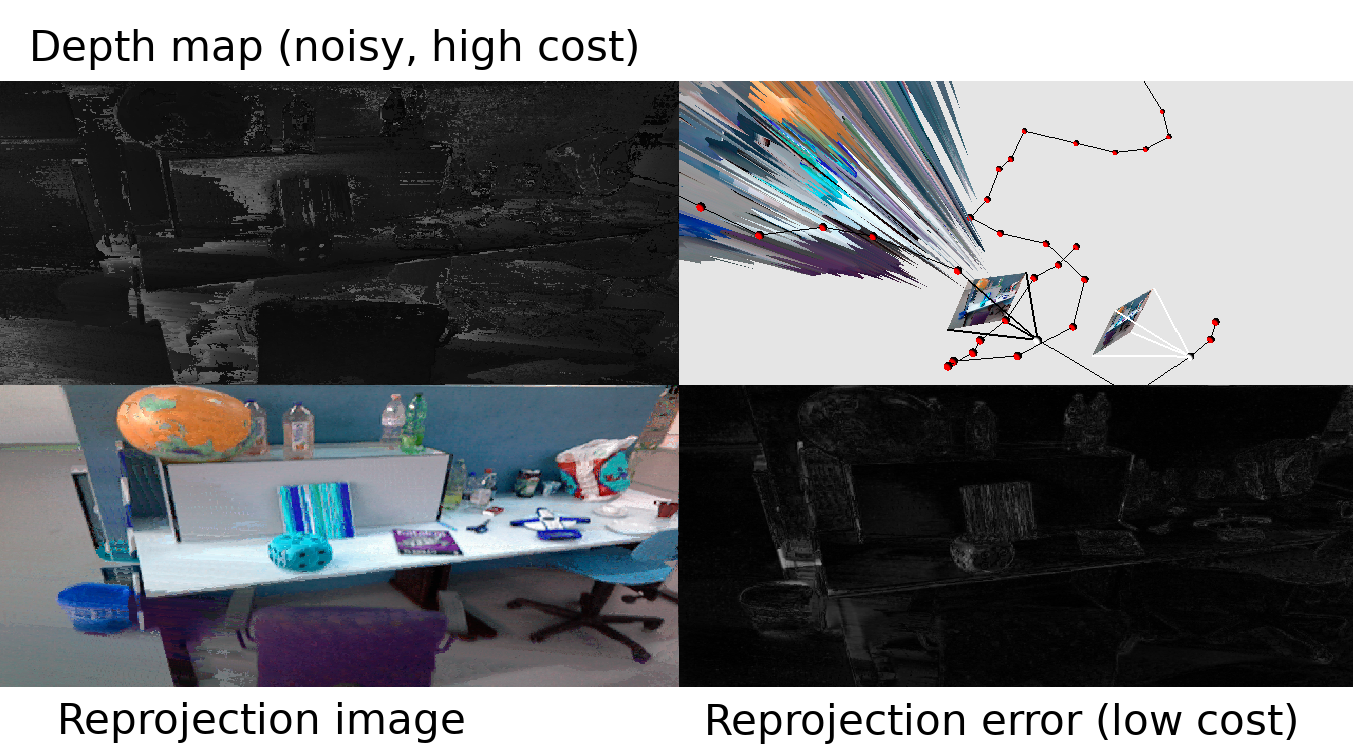
\includegraphics[width=\textwidth]{figures/noisevis_computed_text.png}}
\caption{Brute-force computed, with no regularizer}
\label{noisevis_computed}
\end{subfigure}
\end{figure}

Consider the naive approach of minimizing reprojection error pointwise. For one pixel in frame 1, the depth value parameterizes a ray which
is then reprojected into frame 2. A simple brute-force approach is to search frame 2, along this reprojected ray, for the color which gives minimum
reprojection error.
Figures \ref{noisevis_groundtruth} and \ref{noisevis_computed} visualize the problem with this approach.
Figure \ref{noisevis_groundtruth} displays, using the the ground truth depth map data provided by the Kinect sensor \cite{tum_dataset}, anticlockwise
from the bottom right:
\begin{itemize}
    \item The reprojection image.
    \item The reprojection error.
    \item A 3D view of the depth map placed in world space.
    \item The depth map.
\end{itemize}
Figure \ref{noisevis_computed} displays the same results when using a depth map computed with the naive brute-force algorithm outlined above.

The ground truth reprojection image contains ``coloured shadows'' due to occlusion. These also contribute
to high (white) values in the reprojection error image. The brute-force depth map avoids this occlusion problem.

Consider a pixel in frame 1 corresponding a point which, from the perspective of camera 2, is behind the blue die.
Likely, the line search in frame 2 will find
an unoccluded point, of similar colour, on the table. This, however, gives an unrealistic (and noisy) depth value in general --- compare
the depth images in figures \ref{noisevis_groundtruth} and \ref{noisevis_computed}. Clearly we would like to favour the depth map in
\ref{noisevis_groundtruth}, and this is exactly the reason for the (denoising) regularizing term in \eqref{rof_continuous}.

Due to the freedom of the line search, the brute-force method has achieved low reprojection error (bottom right of figure \ref{noisevis_computed}).
With the ground truth depth map, however, the self-occlusion causes a large amount of reprojection error, which will penalize the cost function
\eqref{rof_continuous}. We would clearly like to minimize the total reprojection error (with the data term), but also keep the depth map ``smooth'' (with the regularizer term), as achieved in \cite{dense_geometry}.
However, it is difficult to choose a good value of $\lambda$ to balance the data and regularizer.

We propose a modification to the method of \cite{dense_geometry}, by removing the 









\section{Comparison of results}

\section{Conclusion}
We have shown the utility of such an algorithm-specific testing framework. It is hoped that, although our reconstructed depth maps are of much lower quality
and our iterative method converges far more slowly than the state of the art reconstruction methods, it is hoped that this is merely an architectural issue.

We have visualised the meaning of the regularizer term used in \cite{dense_geometry}.

\subsection{Future work}
In future research, we would like to implement the much faster, GPU-accelerated multi-grid method of Cremers \cite{dense_geometry},
and perform a systematic comparison of methods from prior research on dense depth reconstruction (\cite{things}).
The main utility of our framework is in the visualization of the effect of parameters such as the regularizer weight $\lambda$ and thresholding
parameter $\theta$.
We would also like to automate comparisons of the results using the rest of the TUM RGB-D dataset \cite{tum_dataset}. A standardized measure of quality
of a depth-from-image-pair algorithm will likely be of great utility. The utility of depth map estimation from colour images is largely in
mobile 3D reconstruction and augmented reality applications. Planned features include an extension of our framework to support the visualisation of volumetric reconstruction algorithms (\cite{largescale}, \cite{volumetric}, \cite{kinectfusion}), by fusing the depth map estimations together into a volumetric data structure.

\section*{References}
\begin{thebibliography}{00}

% \bibitem{b1} G. Eason, B. Noble, and I. N. Sneddon, ``On certain integrals of Lipschitz-Hankel type involving products of Bessel functions,'' Phil. Trans. Roy. Soc. London, vol. A247, pp. 529--551, April 1955.


\bibitem{chambolle}
    Chambolle, A. (2004). An Algorithm for Total Variation Minimization and Applications.
    \textit{Journal of Mathematical Imaging and Vision, 20(1/2), 89--97.}

% TUM and Cremers
\bibitem{dense_geometry}
Cremers, D., St\"uhmer, J., Gumhold, S., (2010). Real-Time Dense Geometry from a Handheld Camera.
    \textit{Lecture Notes in Computer Science, 11--20.}

\bibitem{variational_lectures}
    Cremers, D., Variational Methods in Computer Vision, TUM Department of Infomatics, https://vision.in.tum.de/teaching/online/cvvm (online resource). (Link valid as of June 2021).
\bibitem{largescale}
    Cremers, D., Steinbr\"ucker, F., Kerl, C., St\"urm, J., Large-Scale Multi-Resolution Surface Reconstruction from RGB-D Sequences. In ICCV, 2013.

\bibitem{TUM_volumetric_CPU}
    Cremers, D., Steinbr\"ucker, F., St\"urm, J., Volumetric 3D Mapping in Real-Time on a CPU. In ICRA, 2014.

\bibitem{tum_dataset}
    A Benchmark for the Evaluation of RGB-D SLAM Systems (J. Sturm, N. Engelhard, F. Endres, W. Burgard and D. Cremers), In Proc. of the International Conference on Intelligent Robot Systems (IROS), 2012. 

%----
\bibitem{rof}
    Rudin, L. I., Osher, S., \& Fatemi, E. (1992). Nonlinear total variation based noise removal algorithms.
    \textit{Physica D: Nonlinear Phenomena, 60(1--4), 259--268.}

\bibitem{horn_schunck}
    Horn, B. K., \& Schunck, B. G. (1981). Determining optical flow.
    \textit{Artificial Intelligence, 17(1--3), 185--203.}


\bibitem{tv_optical_flow}
Zach, C., Pock, T., Bischof, H. (2007). A Duality Based Approach for Realtime TV--$L^1$ Optical Flow. 
    \textit{Pattern Recognition: 29th DAGM Symposium, Heidelberg, Germany. Springer. 214-223.}

\bibitem{volumetric}
    Curless, B., Levoy, M. (1996). A Volumetric Method for Building Complex Models from Range Images. In SIGGRAPH, 1996.

\bibitem{kinectfusion}
    R. Newcombe et al. (2011). KinectFusion: Real-Time Dense Surface Mapping and Tracking. Microsoft Research.

\bibitem{szeliski}
    Szeliski, R. (2010). Computer Vision: Algorithms and Applications (Texts in Computer Science). Springer.

\bibitem{aperture_problem}
    aperture problem

\bibitem{variational_calculus}
    Gelfand, I. M., \& Fomin, S. V. (2000). Calculus of Variations (Dover Books on Mathematics). Dover Publications.


\end{thebibliography}

\end{document}
